\documentclass[runningheads]{llncs}

\usepackage[T1]{fontenc}
\usepackage[utf8]{inputenc}
\usepackage{graphicx}
\usepackage{booktabs}
\usepackage{amssymb}
\usepackage{array}
\usepackage{multirow}
\usepackage{url}
\usepackage{color}

\graphicspath{{./}{figs/}{figures/}{./figs/}{./figures/}}
\hyphenation{PhreshPhish CatBoost LightGBM XGBoost SpacePhish}
\newcolumntype{L}[1]{>{\raggedright\arraybackslash}p{#1}}

%% ---------------------------------------------------------------------------
%% FIGURE FILES REQUIRED IN THE SAME OVERLEAF PROJECT AS THIS .tex:
%%     fig1_framework.eps      fig2_attacks.eps
%% Pasting this .tex alone is not enough. If a figure is missing, Overleaf will
%% report "file not found" rather than silently using an older image.
%% Both \includegraphics calls name the .eps file explicitly, so an older
%% fig1_framework.pdf or fig2_attacks.pdf left in the project is never used.
%% Compile with pdfLaTeX; the EPS files are converted automatically.
%%
%% Citations resolve on the SECOND pdflatex pass. If [?] appears, recompile once more.
%% ---------------------------------------------------------------------------
\usepackage[hidelinks,breaklinks=true]{hyperref}
% Springer eBook style for URLs, as in the LNCS sample paper
\renewcommand\UrlFont{\color{blue}\rmfamily}
\hypersetup{pdftitle={Accuracy Is Not Robustness: Realistic Evasion Attacks on
  Phishing Website Detectors},
  pdfauthor={Jatin Kumar, Nisarg Chasmawala, Mohamed Ihmeida, Fuad A. Ghaleb,
  Raouf Abozariba}, pdflang={en}}


\begin{document}

\title{\texorpdfstring{Accuracy Is Not Robustness: Realistic Evasion\\ Attacks on
Phishing Website Detectors}{Accuracy Is Not Robustness: Realistic Evasion Attacks
on Phishing Website Detectors}}

\titlerunning{Accuracy Is Not Robustness}
\authorrunning{J. Kumar, N. Chasmawala et al.}

%% CAMERA-READY VERSION, authors named.
\author{Jatin Kumar\thanks{These authors contributed equally to this work.} \and Nisarg Chasmawala\protect\footnotemark[1] \and Mohamed Ihmeida \and\\
Fuad A. Ghaleb \and Raouf Abozariba}

\institute{Birmingham City University, Birmingham, United Kingdom\\
\email{\{jatin.kumar4, nisarg.chasmawala\}@mail.bcu.ac.uk}\\
\email{\{mohamed.ihmeida, fuad.ghaleb, raouf.abozariba\}@bcu.ac.uk}}

\maketitle

\begin{abstract}
Feature-based machine-learning detectors are the countermeasure most widely
deployed against phishing, and recent studies report 97\% to 99\% accuracy
on standard benchmarks. Three issues limit the value of that figure: (i)
benchmark saturation, so competing methods cannot be separated on shared
datasets; (ii) dataset artefacts, which inflate scores when a single engineered
feature makes a dataset almost trivially separable; and (iii) little evidence on
robustness to attackers who modify a URL to evade detection while preserving its
malicious function. This study evaluates detectors under a constrained evasion
threat model and asks whether properties of a trained model explain differences
in vulnerability. Four tree ensembles, the models most frequently recommended
for this task, and two deep learning models were evaluated, so that no finding
rests on a single model family. The threat model comprises a transfer attack
through a differentiable surrogate and a decision-based attack that sees only
hard labels, on two public datasets of 10,000 and 57,405 pages. Clean
accuracy predicted neither the magnitude of degradation nor the ranking of
models under attack: the tree ensembles' detection on the first dataset fell
from 98.20--98.90\% to between 66.30\% and 69.30\% under a perturbation that left
the second dataset unaffected, and the same architecture left the fewest pages evadable on one dataset
and every page evadable on the other. The difference follows how
far each model relies on features an attacker can modify. Detectors should be evaluated under a well-defined threat model and favour features
that attackers cannot easily manipulate.

\keywords{Phishing detection \and Adversarial machine learning \and Evasion
attacks \and Gradient boosting \and Robustness evaluation \and Cybersecurity.}
\end{abstract}

% =====================================================================
\section{Introduction}
\label{sec:intro}

Phishing remains among the most common methods by which an attacker obtains an
initial foothold within an organisation. The Anti-Phishing Working Group recorded
close to one million distinct attacks in the fourth quarter of 2024
\cite{apwg2024}. The FBI Internet Crime Complaint Center received more
complaints about phishing and spoofing in 2023 than about any other crime type
\cite{ic32023}. Low-cost phishing kits compound the problem, allowing adversaries
with no technical expertise to deploy a convincing replica within minutes.

Most existing solutions are supervised classifiers operating on features
extracted from the URL and the web page. Tree ensembles, and gradient-boosted
ensembles in particular, are the methods most frequently recommended for this
task, and the comparative literature reports accuracies clustered between 97\%
and 99\% \cite{hannousse2021,prasad2024}. However, their robustness against
evasion attacks remains largely unexplored: the few existing studies attack Random
Forest, logistic regression and neural networks, but no gradient-boosted
ensemble \cite{apruzzese2022,montaruli2023}. In such attacks, an adversary can
modify URL and page characteristics to evade detection while preserving the
malicious functionality of the page.

Reporting clean accuracy on a static benchmark, as the studies above do,
overlooks three issues. First, the benchmarks have saturated: once every method
reports performance within a band narrower than seed-to-seed variation, accuracy
no longer discriminates between strong and weak detection models. Second, part of the reported performance is attributable to properties of the
datasets themselves. These datasets represent a fixed and learnable
distribution of attack patterns that can be effectively captured by many machine
learning models. However, this distribution may not fully reflect the diversity,
variability and evolving nature of real-world URLs. On PhiUSIIL \cite{prasad2024}, a single engineered feature dominates the
importance ranking of every model and leaves the data almost trivially separable. Third, and
consequently, a high benchmark score does not establish that a model would resist
an adaptive adversary, because that score is measured on a distribution the
adversary has no reason to respect.

Previous studies, such as \cite{apruzzese2022} and \cite{montaruli2023}, have
demonstrated that adversarial manipulations can effectively reduce the
performance of phishing detection solutions. Neither study, however, evaluated
the gradient-boosted family that dominates deployed feature-based detection, and
neither explained why some detection models survive such attacks while others do
not. This study evaluates phishing detection models under a practical constrained
adversarial evasion model, covering both the gradient-boosted ensembles that are
the most widely used feature-based approaches and two deep learning models. It
further investigates whether properties of trained models can explain differences in their vulnerability to adversarial evasion attacks. Its contributions are the following.

\begin{itemize}
\item A constrained decision-based attack model for tabular phishing detection
models is proposed, in which only attacker-controlled features may be perturbed
and every generated candidate is projected back onto the space of admissible
feature vectors, so that each query corresponds to a page that could plausibly
be constructed.
\item An evaluation methodology is proposed that pairs a surrogate-based transfer
attack with the constrained decision-based attack and applies a single threat
model across two datasets with barely overlapping feature schemas, so that no conclusion
depends on the fidelity of the surrogate model or on one feature-engineering
choice.
\item A feature-importance-based indicator is proposed for explaining differences
in adversarial robustness among phishing detection models, together with a
mitigation strategy based on adversarial training that is validated against a
previously unseen black-box attack.
\end{itemize}

Reported separately from these contributions, the principal findings are that
clean accuracy predicted neither the magnitude nor the ranking of robustness,
that the differences track the proposed reliance indicator, and that adversarial training made black-box evasion costlier on one dataset,
and rarer but cheaper on the other.

Section~\ref{sec:related} reviews related work and identifies the gap,
Section~\ref{sec:method} presents the framework and evaluation design,
Section~\ref{sec:results} reports the results, and Section~\ref{sec:conclusion}
concludes.

% =====================================================================
\section{Related Work}
\label{sec:related}

\subsection{Detecting Phishing with Machine Learning}

Early work showed that lexical and host attributes of a URL alone separate
malicious from benign sites, and feature sets grew to include counts of dots,
hyphens and digits, subdomain depth, character entropy, HTTPS usage and
hyperlink ratios. Tree ensembles occupy the top of most comparative studies
\cite{hannousse2021}, the usual
candidates being Random Forest \cite{breiman2001}, XGBoost \cite{chen2016},
LightGBM \cite{ke2017} and CatBoost \cite{prokhorenkova2018}. These report clean
accuracy on a static split and do not measure behaviour under manipulation. A
separate line of work removes manual feature engineering by learning from the
raw URL string, but the decision still rests on input the attacker composes.

\subsection{Recent Benchmarks and the Base-Rate Problem}

Two datasets released in 2025 sharpen the question. PhreshPhish
\cite{dalton2025} applies temporal splitting with leakage filters and publishes
benchmarks at base rates between 0.05\% and 5\%; its authors report an embedding
classifier at 0.99 average precision, falling to 0.777 at a 0.05\% base rate,
and conclude that much published performance derives from unrealistically high
base rates. URL-Phish \cite{linh2025} provides 111,660 URLs with 22 lexical
features. Two omissions matter: PhreshPhish evaluates no gradient-boosted
ensemble and excludes host-based features to keep latency low, while every URL-Phish feature is attacker-controllable.

\subsection{Adversarial Robustness and Evasion}

Adversarial vulnerability has mostly been studied for differentiable models
such as deep neural networks \cite{madry2018}, and its extension to phishing raises two complications. Tree
ensembles provide no gradients, so an attack must transfer from a surrogate
\cite{papernot2017} or search without gradients \cite{brendel2018,chen2020}.
The second complication is more basic: an $L_p$ perturbation in feature space
need not correspond to any object an attacker can construct, a gap formalised as
feature space against problem space \cite{pierazzi2020}.
Within phishing detection, SpacePhish \cite{apruzzese2022} reports that
inexpensive website-space edits degrade detection significantly while a few
models resist, and Raze to the Ground \cite{montaruli2023} evades those models
within roughly thirty queries using functionality-preserving HTML manipulations.
For comparison, HopSkipJump \cite{chen2020} improves query efficiency by
estimating the boundary gradient direction from binary responses, and
mixed-integer formulations compute provably minimal perturbations for tree
ensembles at higher cost. The attack proposed here belongs to the same
decision-based family as the former while enforcing validity constraints neither
addresses directly.

\subsection{Positioning of the Present Study}
\begin{table}[!htbp]
\centering
\caption{The closest prior studies are set against the present one. TB, SB and
DB denote transfer-based, score-based and decision-based attacks, and blind edits
are made without querying the detector; the final column states the principal
limitation addressed here.}
\label{tab:gap}
\footnotesize
\setlength{\tabcolsep}{2.6pt}
\begin{tabular}{lccccL{2.3cm}}
\toprule
Study & Deep & Attack & Cross- & Reliance & Principal \\
      & models & type & dataset & analysis & limitation \\
\midrule
Hannousse \& Yahiouche \cite{hannousse2021} & no & none & no & no & accuracy only \\
Prasad \& Chandra \cite{prasad2024}         & no & none & no & no & leakage-prone \\
Apruzzese et al.\ \cite{apruzzese2022}      & yes & blind & yes & no & other detectors \\
Montaruli et al.\ \cite{montaruli2023}      & yes & SB & no & no & no explanation \\
Dalton et al.\ \cite{dalton2025}            & yes & none & no & no & no boosting \\
Linh \& Hung \cite{linh2025}                & yes & none & no & no & all mutable \\
\midrule
\textbf{This study} & \textbf{yes} & \textbf{TB + DB} & \textbf{yes} & \textbf{yes} & --- \\
\bottomrule
\end{tabular}
\end{table}


Benchmark accuracy is also fragile under distribution shift. URL classifiers
degrade substantially on URLs drawn from sources unlike their training data, and
the features on which a model relies are often specific to a single dataset.
Table~\ref{tab:gap} sets the closest prior work against the present study.
Against this background, the study differs on four counts. Where Hannousse
and Yahiouche \cite{hannousse2021} and Prasad and Chandra \cite{prasad2024}
compare detectors without attacking them, and where SpacePhish
\cite{apruzzese2022} and Raze to the Ground \cite{montaruli2023} attack detectors
other than gradient-boosted ones, both are combined here under a constraint set built for URL
and page validity. A transfer attack is run alongside a constrained
decision-based attack, so that no conclusion depends on surrogate fidelity. A
single threat model is applied to two datasets with barely overlapping schemas, and
robustness is shown not to transfer between them. Finally, the observed gap is explained by a property measurable on a trained
model, namely its reliance on features that are harder for an attacker to
control.

% =====================================================================
\section{Methodology}
\label{sec:method}

Figure~\ref{fig:method} presents the experimental framework, which proceeds in
five stages. Stage~1 prepares both datasets and partitions the feature set.
Stage~2 trains the detection models, the surrogate model used by the transfer
attack, and the validity projection constraining every generated sample. Stage~3
generates adversarial samples using two attacks, each drawing on a different
Stage~2 component: the transfer attack uses the surrogate model's gradients, the
decision-based attack queries the trained models directly, and both pass every
candidate through the validity projection. Stage~4 measures clean performance,
robustness and feature reliance from the Stage~3 outputs, and derives the problem-space evasion recipe reported in
Section~\ref{sec:res-defence}, which expresses an evasion as
concrete page edits. Stage~5 retrains one
model on augmented data and returns it to Stage~3, along the dashed path, for
re-evaluation by an attack that played no part in its training.

\begin{figure}[!htbp]
\centering
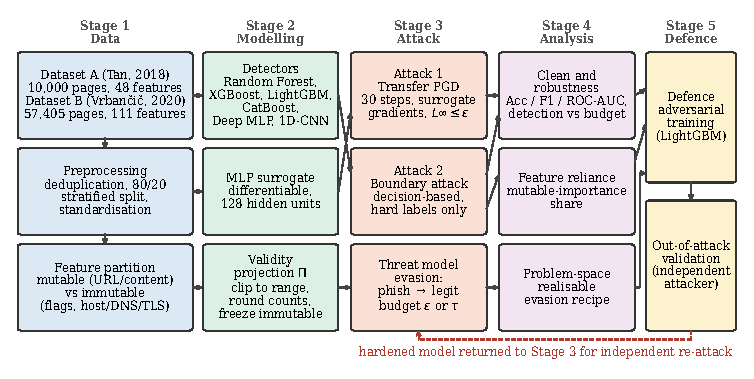
\includegraphics[width=\textwidth,
  alt={Flowchart of the five-stage framework, read left to right: data, modelling, attack, analysis and defence. Each stage feeds the next. The two attacks in Stage 3 draw on different Stage 2 components, the transfer attack on the surrogate model and the decision-based attack on the trained detectors, and a dashed arrow returns the retrained model from Stage 5 to Stage 3 to be attacked again by an attacker it was not trained against.}]{fig1_framework.eps}
\caption{The experimental framework}
\label{fig:method}
\end{figure}

\subsection{Threat Model}
\label{sec:method-threat}

This study assumes an attacker who operates at test time and seeks to have a
phishing page misclassified as legitimate, with no access to the internals of
the target classifier. Only features determined by the URL string
and the markup the attacker authors may be modified. Poisoning and model
extraction fall outside the scope of this paper.

\paragraph{Goal.} Given a phishing sample $x$ that the target classifier $f$ classifies correctly,
the adversary seeks a modified $x'$ that $f$ classifies as legitimate and that
remains deployable. The phishing class is targeted because an evasion adversary
wants malicious pages classified as benign; false positives matter
operationally but are not its objective.
Reported detection is recall on the phishing class under attack, measured over
all held-out phishing samples supplied to the attack.

\paragraph{Knowledge.} The transfer attacker cannot query the original target
classifier. It trains a differentiable substitute, here on the same training split as
the detectors, and relies
on adversarial examples transferring between models \cite{papernot2017}. The
decision-based attacker is strictly black-box and observes only the hard label
returned by the original target classifier. The second setting is the more
conservative of the two for a defender, because its outcome does not depend on
how closely the substitute happens to approximate the target: any degradation it reports is attributable to
the target classifier itself.

\paragraph{Capability.} Only attacker-controllable features may be perturbed,
namely those determined by the URL string and the markup the attacker writes.
Features reflecting hosting infrastructure remain fixed, and every candidate must
be an admissible feature vector. Let $M$ denote the set of indices of
attacker-controllable features, $[\ell_j, u_j]$ the range of feature $j$ observed
in the training split, $\delta$ the perturbation applied to the original sample,
and $\Pi$ the validity projection. Then
\begin{equation}
x' = \Pi(x + \delta), \quad \delta_j = 0 \;\; \forall j \notin M, \quad
\|\delta\|_p \le b,
\label{eq:threat}
\end{equation}
\begin{equation}
\Pi(z)_j = \left\{
\begin{array}{ll}
\mathrm{round}\big(\mathrm{clip}(z_j, \ell_j, u_j)\big) & \mbox{if } j \mbox{ is integer-valued},\\[2pt]
\mathrm{clip}(z_j, \ell_j, u_j) & \mbox{otherwise.}
\end{array}\right.
\label{eq:proj}
\end{equation}

The attack budget $b$ bounds how far a generated sample may move from the
original page, in standardised units so that one value means the same across
features on different scales. Two norms are used: $\|\delta\|_\infty$, the
largest change to any single feature, bounded by $\epsilon$ for the transfer
attack, and $\|\delta\|_2$, the Euclidean length of the whole perturbation
vector, bounded by $\tau$ for the decision-based attack. Concretely, on
Dataset~A a budget of $\epsilon = 0.05$ corresponds to changing the length of a
URL by roughly two characters, while $\tau = 2.0$ corresponds to moving ten
mutable features by about 0.63 standardised units each.
The budget is not a claim that larger edits are impossible; it traces how
detection degrades as the attacker moves away from the original page. The lower
end corresponds to an edit too small to matter operationally, one or two characters in a URL; the upper end to one large enough that the page loses what made it
convincing. Values are spaced finely near zero because almost all degradation on
Dataset~A occurs at the smallest non-zero budget, which a coarser grid would have
hidden.

The projection $\Pi$ enforces per-feature ranges and integrality but does not
encode every dependency between related features, for instance exact consistency
between a URL string and all counts derived from it. Generated samples are
therefore admissible with respect to the constraints imposed, and are not claimed
to be fully realistic web pages in every respect.

\subsection{Datasets and Feature Partition}
\label{sec:data}

Two public datasets with barely overlapping schemas were used, so a conclusion
appearing on both is unlikely to be an artefact of one feature-engineering
choice. Dataset~A \cite{tan2018} comprises 10,000 balanced
instances across 48 numeric URL and page-content features; it has been
benchmarked extensively, which is precisely why clean accuracy on it conveys
little. Dataset~B \cite{vrbancic2020} contains 58,645 instances, reduced to
57,405 after removing exact duplicates, across 111 features whose schema adds
host, DNS, registration-time and TLS attributes. It is six times larger, originates
from a different source, and contains signals that an attacker cannot fabricate
by authoring a page, which makes it a demanding external check.

The partition between attacker-controllable features and the rest carries most
of the weight in this design. A feature is controllable when the attacker sets
it by choosing a URL and writing markup. Features reflecting hosting
infrastructure, registration history or certificate state are harder to control:
they can be changed, but at a cost and delay that authoring a page does not
incur. The two groups are referred to below as mutable and immutable, with that
qualification understood. On Dataset~A the 19 mutable
features are URL-lexical counts and lengths together with three content ratios
covering external hyperlinks, external resources and null self-redirects, and the
29 immutable features are URL and page indicators, such as the at-symbol,
IP-address, form and popup flags, plus six derived risk terms. Dataset~A has no
infrastructure features, and freezing these indicators, most of which the URL or
markup could change, makes its results a lower bound on vulnerability. On Dataset~B the 76 mutable features comprise all per-segment character
counts over the URL, directory, file and parameter components plus the three
segment lengths, while the 35 immutable features describe the domain name
and its infrastructure, including domain activation and expiration times, name-server and mail-server counts, hostname time-to-live, TLS
certificate state and autonomous-system identifiers.

Features were standardised using training-split statistics alone, and the
validity projection $\Pi$ takes per-feature ranges from the training split and an
integer mask from the full dataset, which keeps count features whole. A static stratified
split was used because neither dataset ships reliable collection timestamps. This
is a genuine limitation: phishing campaigns evolve, so a model trained on past
pages and tested on future ones would face concept drift and adversarial
adaptation at once, and a random split measures neither. The absolute rates
reported here are therefore an upper bound on performance under temporal
evaluation. The comparison between models is less sensitive to this, since all
models are measured under identical conditions.

\subsection{Detection Model Training}
\label{sec:models}

Six detection models were trained on an 80/20 stratified split with settings
identical across both datasets. Four are tree ensembles: Random Forest with 250
trees and $\sqrt{d}$ features per split, where $d$ is the number of features;
XGBoost with 350 rounds, depth 6, learning rate 0.04, row and column subsampling
of 0.9 and 0.8 and $L_2$ regularisation $\lambda = 1.0$; LightGBM with 400 rounds,
63 leaves and no depth limit, with the same learning rate, column subsampling
and regularisation; and CatBoost with 350 iterations, depth 6, learning
rate 0.05 and $L_2$ leaf regularisation 3.0. These were selected because they are
the methods most frequently recommended for feature-based phishing detection in
the comparative literature \cite{hannousse2021,prasad2024}, and therefore
represent the family most likely to be deployed. Hyperparameters follow the values reported in those comparative studies and were
not tuned for this study. Tuning each model to its own optimum would let a robustness
difference reflect search effort as easily as the model or the feature
representation, so the settings are held fixed and identical across both datasets.

Two deep learning models were added so that no conclusion is an artefact of a
single model family. The first is a deep multilayer perceptron with three hidden layers of
256, 128 and 64 ReLU units, trained with Adam and early stopping. The second is a one-dimensional convolutional network with two convolutional
blocks, global max pooling and a dense head, whose inductive bias differs
because convolution assumes local structure among adjacent features. It was trained on each dataset's
full training split with the number of gradient steps held near 800, so the
larger dataset received no extra optimisation.

Because the tree ensembles are not differentiable, a separate multilayer
perceptron with one hidden layer of 128 ReLU units (gradient descent,
learning rate 0.05, 200 epochs, batch size 256) was also trained to act as the surrogate model for the transfer attack. It
was never evaluated as a detection model.

\subsection{Adversarial Evasion Attack Generation}
\label{sec:method-attacks}

\paragraph{Transfer attack.} Projected gradient descent (PGD), an iterative
first-order attack that repeatedly takes a small step in the direction that
increases the model's loss and then projects the result back into the permitted
region, was run for 30 steps against the surrogate model, and the resulting
perturbations were transferred to each detection model. Each step restricts the
perturbation to mutable features, clips it to the $L_\infty$ ball of radius
$\epsilon$, and passes it through $\Pi$, with immutable coordinates reset after
every step. The budget was swept over
$\epsilon \in \{0, 0.05, 0.1, 0.2, 0.3, 0.5, 0.75, 1.0\}$.

\paragraph{Decision-based Boundary attack.} To remove any dependence on surrogate
fidelity, a constrained gradient-free attack in the Boundary family
\cite{brendel2018} was implemented, operating on hard labels alone. A warm-start
phase performs a random search over mutable features at increasing magnitudes and
retains the smallest-$L_2$ point that changes the label; a refinement phase moves
that point back toward the original while remaining on the legitimate side of the
decision boundary, with small orthogonal moves to escape ridges. Every candidate
passes through $\Pi$, so each query corresponds to an admissible page. The attack
terminates when the refinement budget of 100 iterations is exhausted, giving at
most 355 queries per sample; steps that fail to improve the best perturbation are
discarded and the step size is reduced when the improvement rate falls below
30\%. Reported per model are the fraction of pages evadable within admissible
ranges, the median $L_2$ required, and surviving detection against $\tau$; a page
the model already misclassifies counts as evaded at zero cost.

\subsection{Feature-Reliance Analysis}
\label{sec:method-reliance}

For Random Forest and LightGBM on each dataset, the built-in feature importances
$I_j$ (mean impurity decrease and split counts respectively) were normalised and
summed over the mutable set $M$, giving a mutable-importance share
$S_{\mathrm{mut}}$, computed on refits without LightGBM's subsampling and
regularisation. This links a black-box robustness measurement to a quantity
readable directly from a trained model. Because built-in importance is
known to favour correlated and high-cardinality features, permutation importance
was computed as a check, using three repeats on up to 3,000 held-out pages and scoring by accuracy.

\subsection{Adversarial Training and Robustness Evaluation}
\label{sec:method-defence}

The LightGBM-based classifier was retrained using an augmented training set
containing transfer-PGD adversarial examples of the training phishing samples,
generated across $\epsilon \in \{0.05, 0.1, 0.15, 0.2, 0.3, 0.4, 0.5\}$, then
evaluated twice: under the transfer attack against which it was trained, and
under the independent decision-based attack along the dashed path in
Figure~\ref{fig:method}. The second evaluation distinguishes genuine robustness
gains from memorisation of the training-time attack. To account for variability
arising from the data split, model initialisation and attack randomness, the four ensembles on Dataset~A were rerun under five random seeds, with
standard deviations of at most 0.33 percentage points in clean accuracy and 4.3
in detection rate at any budget; the tables report seed~42. All computation ran on the CPU of a Google Colab
runtime, a single-seed pipeline requiring 122
seconds on Dataset~A and 343 seconds on Dataset~B.

% =====================================================================
\section{Results and Discussion}
\label{sec:results}

\subsection{Experiments}
\label{sec:res-setup}

Dataset~A was split into 8,000 training and 2,000 test instances, Dataset~B into
45,924 and 11,481. The transfer attack used every held-out phishing page, 1,000 in Dataset~A, and
the decision-based attack the first 400 for each model, balancing precision
against its query cost:
at 400 samples a detection rate is estimated to within roughly five percentage
points at 95\% confidence, far finer than the effects measured. The pipeline uses scikit-learn, XGBoost, LightGBM and CatBoost; the
surrogate, the CNN and both attacks are written in NumPy.

\subsection{Clean Performance Evaluation}
\label{sec:res-clean}

Table~\ref{tab:main} reports clean performance on the unmodified test set
alongside the robustness figures discussed in Section~\ref{sec:res-boundary}.
All four ensembles reach at least 98.50\% accuracy on Dataset~A with ROC-AUC above
99.80\%, and on Dataset~B accuracy falls between 94.55\% and 95.80\%. Under a
conventional reading every model performs well and the choice between them is
immaterial. The rest of Section~\ref{sec:results} shows why that reading misleads.

\begin{table}[!htbp]
\centering
\caption{Accuracy, $F_1$ and ROC-AUC are percentages on the unmodified test set. Evadable is
the percentage of phishing pages that can be evaded within admissible ranges, and
median $L_2$ the perturbation required, where a larger value indicates greater
robustness. Detection against the attack budget is plotted in Figure~\ref{fig:attacks}.}
\label{tab:main}
\footnotesize
\setlength{\tabcolsep}{3.2pt}
\begin{tabular}{llccccc}
\toprule
& & \multicolumn{3}{c}{Clean evaluation} & \multicolumn{2}{c}{Under attack} \\
\cmidrule(lr){3-5}\cmidrule(lr){6-7}
Dataset & Model & Accuracy & $F_1$ & ROC-AUC & Evadable & Median $L_2$ \\
\midrule
\multirow{6}{*}{A: Tan}
 & Random Forest & 98.50 & 98.50 & \textbf{99.89} & 94.75 & \textbf{2.64} \\
 & XGBoost       & \textbf{98.75} & \textbf{98.75} & 99.88 & 99.00 & 1.85 \\
 & LightGBM      & 98.55 & 98.55 & 99.88 & 99.00 & 2.03 \\
 & CatBoost      & 98.65 & 98.65 & 99.85 & 95.00 & 1.58 \\
 & Deep MLP      & 97.40 & 97.39 & 99.67 & 98.00 & 1.85 \\
 & 1D-CNN        & 90.45 & 90.66 & 95.96 & \textbf{84.25} & 2.10 \\
\midrule
\multirow{6}{*}{B: Vrban\v{c}i\v{c}}
 & Random Forest & 95.71 & 95.99 & 99.16 & \textbf{57.75} & 5.86 \\
 & XGBoost       & 94.98 & 95.28 & 99.02 & 90.00 & 5.85 \\
 & LightGBM      & \textbf{95.80} & \textbf{96.05} & \textbf{99.22} & 80.75 & 5.71 \\
 & CatBoost      & 94.55 & 94.88 & 98.88 & 81.25 & \textbf{5.96} \\
 & Deep MLP      & 94.87 & 95.13 & 98.63 & 81.75 & 4.38 \\
 & 1D-CNN        & 81.64 & 81.63 & 91.34 & 100.00 & 2.78 \\
\bottomrule
\end{tabular}
\end{table}

\subsection{Performance Evaluation under Transfer Attacks}
\label{sec:res-transfer}

Figures~\ref{fig:attacks}(a) and (b) show detection as the transfer attacker's
budget increases, and the datasets behave very differently. Dataset~A collapses:
perturbing mutable features by 0.05 standardised units reduces detection from
98.20--98.90\% to between 66.30\% and 69.30\% across the four ensembles, after
which every curve is flat. The deep models degrade far more slowly, from 97.20\%
to 66.20\% and from 92.70\% to 74.80\% across the full range. Detection on Dataset~B declines gradually, unchanged at $\epsilon = 0.05$ and
still between 59.60\% and 88.21\% at $\epsilon = 1.0$, the lower figure
belonging to the convolutional network and the upper to Random Forest. Since the model families and their clean accuracy are
comparable, the difference is attributable to the feature representation rather
than to the learning algorithm.


The degradation is clearer in counts. Dataset~A contributes 2,000 test pages,
half of them phishing. Under clean evaluation the LightGBM-based classifier
misclassifies 29, the deep multilayer perceptron 52 and the convolutional
network 191. At $\epsilon = 0.3$, 309 of the 1,000 phishing pages pass the
LightGBM-based classifier as legitimate, against 148 and 86 for the two deep
models, in every case within admissible ranges.

\begin{figure}[!htbp]
\centering
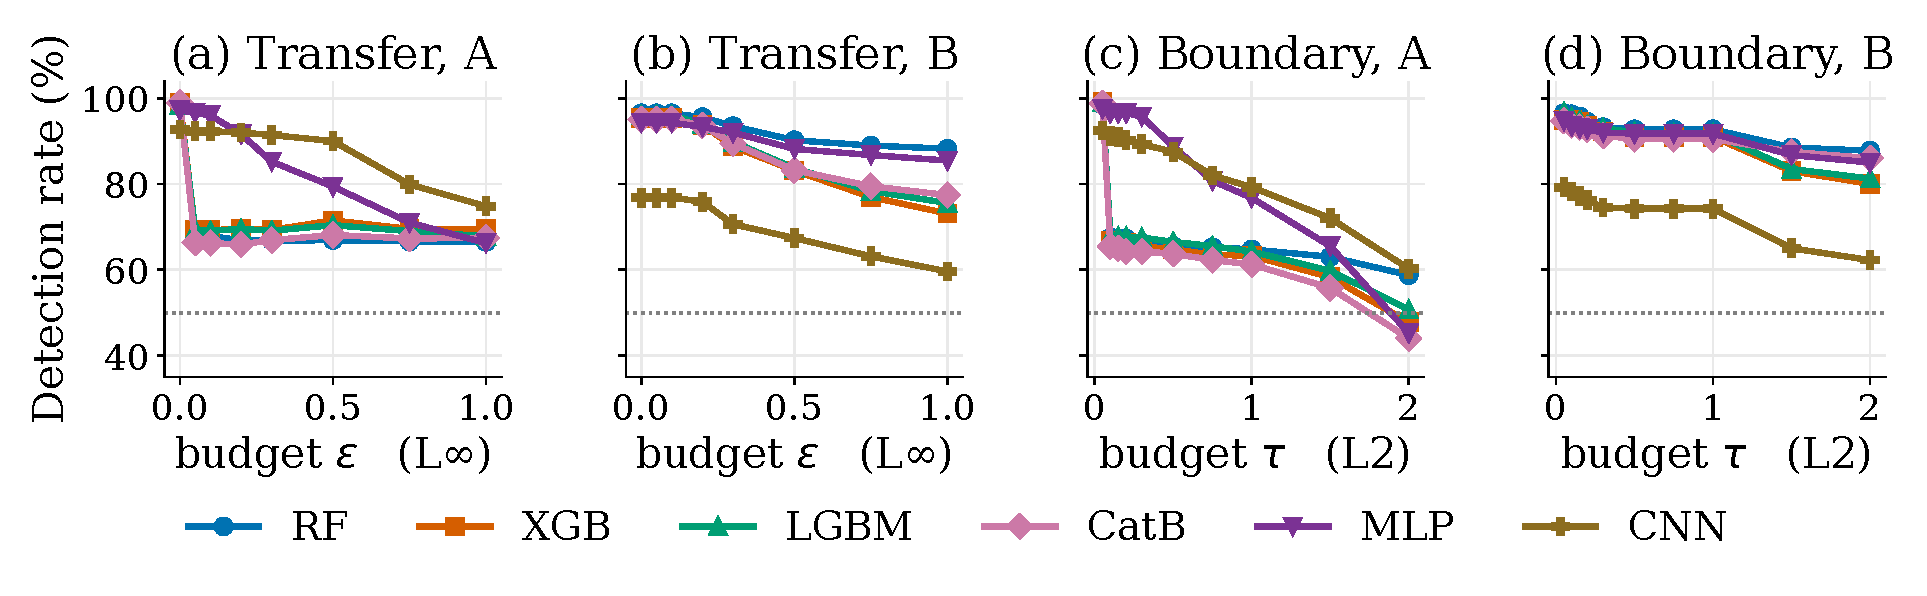
\includegraphics[width=\textwidth,
  alt={Four line charts of phishing detection rate for six detectors as the attack budget grows: the transfer attack on Datasets A and B, then the Boundary attack on Datasets A and B. On Dataset A, transfer detection for the four tree ensembles drops from about 98\% to between 66\% and 69\% at the smallest non-zero budget and stays flat, and the Boundary attack brings them from about 99\% to between 65\% and 68\% by its second budget; on Dataset B both attacks lower detection gradually. At the largest Boundary budget, detection is between 44\% and 60\% on Dataset A but between 62\% and 88\% on Dataset B.}]{fig2_attacks.eps}
\caption{Panels (a) and (b) show the phishing detection rate under transfer PGD
against the $L_\infty$ budget $\epsilon$ on Datasets~A and B; panels (c) and (d) show it
under the constrained Boundary attack against the $L_2$ budget $\tau$.
Table~\ref{tab:main} reports evadability and median perturbation.}
\label{fig:attacks}
\end{figure}

\subsection{Performance Evaluation under Decision-Based Attacks}
\label{sec:res-boundary}

A reasonable objection is that the surrogate might have matched these models
unusually well, so the Boundary attack, which observes neither gradients nor
probabilities, was run as an independent check; Figures~\ref{fig:attacks}(c) and
(d) plot surviving detection against the $L_2$ budget. It reaches the same
conclusion. At the largest budget plotted, $\tau = 2.0$, detection falls to
between 44\% and 60\% on Dataset~A but stays between 62\% and 88\% on
Dataset~B. The separation between the datasets
persists without gradient information, and on Dataset~B many pages could not
be evaded at all: for Random Forest only 57.75\% are evadable, so for over 40\%
of phishing pages the attack found no modification of the 76 mutable features
that alters the verdict.


Two details sharpen the point. Evasion is roughly three times cheaper on
Dataset~A than on Dataset~B, and within Dataset~A the models order themselves
clearly by robustness even though clean accuracy does not separate them: by
median $L_2$, Random Forest is the most resistant at 2.64 and CatBoost the least
at 1.58, a 67\%
difference in the perturbation an attacker must apply, which accuracy conceals
entirely. On
Dataset~B the tree ensembles demand a similar median perturbation, between 5.71
and 5.96, so even the robustness ranking is dataset-dependent. The two
deep learning models sharpen that dependence. On Dataset~A the convolutional network is
the hardest of the six to evade by evadable share, with 84.25\% of pages evadable against 94.75\% to 99.00\% for the
ensembles, whereas on Dataset~B, where it already misses 23.2\% of phishing pages before
any attack, every page is evadable at a median cost of 2.78,
the lowest on that dataset. The same architecture therefore moves from hardest
to easiest to evade across the two datasets, which is hard to reconcile with any account
attributing robustness to the learning algorithm. On Dataset~A both deep models also resist
the transfer attack more effectively than the ensembles, retaining 96.60\% and
92.30\% detection at $\epsilon = 0.05$. This is likely an artefact of the attack:
the surrogate is a network with a single hidden layer, and its gradients need
not transfer to deeper or convolutional architectures, which is why the
decision-based attack is the fairer comparison.

\subsection{Explaining the Difference in Robustness}
\label{sec:res-reliance}

On the fragile Dataset~A the LightGBM-based classifier draws 76.6\% of its built-in importance from mutable features against a median
$L_2$ of 2.03, whereas on Dataset~B it draws 26.9\% and requires 5.71, relying
instead on immutable features of the domain and its hosting. Random Forest sits
at 59.5\% and 63.0\%, evading at 2.64 and 5.86. Where discriminative power resides in features the attacker controls, the input
can be moved across the boundary; where it does not, evasion is bounded however
the URL is rewritten. Random Forest is a partial exception, with
a similar mutable share on both datasets yet the highest median $L_2$ on
Dataset~A, which is consistent with the wider claim: robustness is governed by
where the signal concentrates, and a forest distributes importance thinly while
boosting concentrates it.

Permutation importance was computed as a check, because built-in
importance favours correlated and high-cardinality features. On Dataset~A it
returns 55.8\% for Random Forest and 66.2\% for LightGBM, preserving the
ordering at a smaller contrast; on Dataset~B it returns 33.2\% and 46.0\%,
reversing the built-in ordering. The direction of the central comparison
survives, since LightGBM still falls from 66.2\% to 46.0\%, but the magnitude
is smaller than the built-in figures suggest. The permutation estimates are
therefore the conservative reading, and the disagreement between measures is
itself a reason to treat any single importance-based indicator with caution.


\subsection{Realisability and Adversarial Training}
\label{sec:res-defence}

Feature-space perturbations matter only if they describe pages an attacker could
construct. Starting from a Dataset~A page that the LightGBM-based classifier
assigned a phishing probability of
0.987, chosen for illustration because a few groups of edits evade it, each
group moved mutable features toward the median across legitimate training
pages. Removing sensitive keywords changed nothing, since that feature
already sat at the median; normalising the external-link and self-redirect
ratios then reduced the probability to 0.005 in one step and reversed the
verdict, changing three values in total, all under the attacker's control at
authoring time.

Adversarial training was then evaluated as a mitigation strategy
(Table~\ref{tab:defense}) in a run limited to the four ensembles with the same
seed, whose LightGBM baseline is within 0.2 points of the main run. On Dataset~A it performed well against the attack it
was trained on, and clean accuracy barely moved, from 98.55\% to 98.65\%. Transfer detection at $\epsilon = 0.3$
recovered from 69.30\% to 99.70\%, and the median $L_2$ demanded by the
independent Boundary attack increased from 2.03 to 2.84. That final figure
carries the greatest weight, since the Boundary attack played no part in
training. On Dataset~B the same procedure raised transfer detection to
99.90\%, yet the independent Boundary attack still evaded 27.25\% of pages, down
from 80.75\%, and the median $L_2$ of those evasions fell from 5.71 to 3.70.
The main run, which hardens its own copy, agrees: there the median $L_2$
rose to 2.97 on Dataset~A and fell to 3.84 on Dataset~B. A mitigation strategy must therefore be evaluated against an attack
other than the one used to construct it.

\begin{table}[!htbp]
\centering
\caption{Arrows run from the original LightGBM-based classifier to the
adversarially trained one, with transfer detection at $\epsilon = 0.3$ and black-box
median $L_2$ under the independent decision-based attack. All values come from
the run limited to the four ensembles.}
\label{tab:defense}
\small
\setlength{\tabcolsep}{6pt}
\begin{tabular}{lccc}
\toprule
Dataset & Clean acc.\ (\%) & Transfer det.\ (\%) @ $\epsilon{=}0.3$ & Black-box median $L_2$ \\
\midrule
A: Tan              & $98.55 \rightarrow 98.65$ & $69.3 \rightarrow 99.7$ & $2.03 \rightarrow 2.84$ \\
B: Vrban\v{c}i\v{c} & $95.80 \rightarrow 95.03$ & $89.8 \rightarrow 99.9$ & $5.71 \rightarrow 3.70$ \\
\bottomrule
\end{tabular}
\end{table}

\subsection{Discussion}
\label{sec:discussion}

Across both datasets clean accuracy remained high while conveying little of
practical value, giving no indication of the magnitude of degradation, of how
models would rank under attack, or of the effect of a mitigation strategy.
Robustness requires direct measurement under a stated threat model, reported
alongside accuracy.

Features derived from the URL string and markup are precisely those an adversary
rewrites, so a model concentrating its signal there needs only a small
perturbation to evade. Features grounded in hosting infrastructure, registration
history and TLS state cannot be produced by authoring a page, and bound what a
lexical-only attacker can achieve. Auditing the mutable-importance share of a
candidate model is therefore recommended; where it is high, either infrastructure
signals should be added or the reliance regularised. One deployment tension is
worth naming: PhreshPhish \cite{dalton2025} excludes host-based features because
retrieving them adds latency, which suits real-time blocking but, on this
evidence, reduces robustness. Results should also be read with the deployment
base rate in mind, since both datasets are near-balanced whereas phishing is rare
in operation.

Adversarial training improved robustness. However, the decision-based attacker
it had not seen still evaded more than a quarter of Dataset~B pages, at a lower
median cost than before, which reporting the training-time attack alone would
have concealed. A robustness claim becomes credible only after
adaptive, or at minimum independent, evaluation.

% =====================================================================
\section{Conclusion}
\label{sec:conclusion}

This study evaluated six phishing detection models, four tree ensembles and two
deep learning models, on two public datasets under a constrained adversarial
evasion threat model, combining a surrogate-based transfer attack with a
decision-based attack using hard labels alone. Clean accuracy of the four ensembles was uniformly
high, between 94.55\% and 98.75\%, yet robustness diverged: their detection on
Dataset~A fell from 98.20--98.90\% to between 66.30\% and 69.30\% under a perturbation that left Dataset~B unaffected, and clean
accuracy anticipated neither outcome. The divergence follows the extent to which
a model relies on attacker-controllable features, and three realisable edits
reduced a page scored at 0.987 to a legitimate verdict. Adversarial training
raised the median black-box evasion cost from 2.03 to 2.84 on Dataset~A, and on
Dataset~B cut evadable pages from 80.75\% to 27.25\% while making the remaining
evasions cheaper. The
study contributes a constrained decision-based attack model that enforces page
validity on every query, an evaluation methodology applying a single threat model
across two datasets with barely overlapping schemas, and a feature-importance-based
indicator for explaining differences in robustness, together with a mitigation
strategy evaluated against an attack it was not trained on.

Three limitations bound these conclusions. Both datasets were split at random
because neither carries collection timestamps, so the reported rates are an
upper bound under concept drift; validation is confined to feature space under
box and integrality constraints, so a problem-space attack regenerating complete
pages would be stronger evidence; and the reliance indicator was estimated from built-in and permutation importance,
which disagree in magnitude and, on Dataset~B, in ranking, so it is a coarse
guide only. The practical implications are
nonetheless concrete. A detection model should not be selected on clean accuracy
alone.
The mutable-importance share can be computed from any trained model before
deployment, and where it is high the representation should be supplemented with
signals an attacker cannot manufacture, such as domain age, name-server counts
or certificate state. Any hardening claim should be validated against an attack
the defence was not trained on. Future work will address the first two
limitations through temporal evaluation on a timestamped corpus and an end-to-end problem-space attack, and will widen the attack battery on the newer
datasets at realistic base rates.

\subsubsection{Reproducibility.}
The notebooks, which retrain and save every model, and the result files are
available at
\begin{sloppypar}
\noindent\url{https://github.com/Jatinkumar78/Accuracy-Is-Not-Robustness}
\end{sloppypar}

% =====================================================================
\begin{credits}
\subsubsection{\discintname}
The authors have no competing interests to declare that are relevant to the
content of this article.
\end{credits}

\begin{thebibliography}{99}

\bibitem{apwg2024}
Anti-Phishing Working Group: Phishing activity trends report, fourth quarter
2024. APWG (2025)

\bibitem{apruzzese2022}
Apruzzese, G., Conti, M., Yuan, Y.: SpacePhish: the evasion-space of adversarial
attacks against phishing website detectors using machine learning. In: Annual
Computer Security Applications Conference (ACSAC), pp.~\mbox{171--185} (2022)

\bibitem{breiman2001}
Breiman, L.: Random forests. Machine Learning \textbf{45}(1), 5--32 (2001)

\bibitem{brendel2018}
Brendel, W., Rauber, J., Bethge, M.: Decision-based adversarial attacks: reliable
attacks against black-box machine learning models. In: International Conference
on Learning Representations (ICLR) (2018)

\bibitem{chen2020}
Chen, J., Jordan, M.I., Wainwright, M.J.: HopSkipJumpAttack: a query-efficient
decision-based attack. In: IEEE Symposium on Security and Privacy, pp.~\mbox{1277--1294} (2020)

\bibitem{chen2016}
Chen, T., Guestrin, C.: XGBoost: a scalable tree boosting system. In: ACM SIGKDD
International Conference on Knowledge Discovery and Data Mining, pp.~\mbox{785--794}
(2016)

\bibitem{dalton2025}
Dalton, T., Gowda, H., Rao, G., Pargi, S., Hadj Khodabakhshi, A., Rombs, J.,
Jou, S., Marwah, M.: PhreshPhish: a real-world, high-quality, large-scale phishing
website dataset and benchmark. arXiv:2507.10854v1 (2025)

\bibitem{ic32023}
Federal Bureau of Investigation, Internet Crime Complaint Center: 2023 Internet
crime report. FBI IC3 (2024)

\bibitem{hannousse2021}
Hannousse, A., Yahiouche, S.: Towards benchmark datasets for machine learning
based website phishing detection: an experimental study. Engineering Applications
of Artificial Intelligence \textbf{104}, 104347 (2021)

\bibitem{ke2017}
Ke, G., Meng, Q., Finley, T., Wang, T., Chen, W., Ma, W., Ye, Q., Liu, \mbox{T.-Y.}:
LightGBM: a highly efficient gradient boosting decision tree. In: Advances in
Neural Information Processing Systems (NeurIPS), pp.~\mbox{3146--3154} (2017)

\bibitem{linh2025}
Linh, D.M., Hung, T.C.: A feature-engineered dataset of benign and phishing URLs
for machine learning and large language models evaluation. Data in Brief
\textbf{63}, 112162 (2025)

\bibitem{madry2018}
Madry, A., Makelov, A., Schmidt, L., Tsipras, D., Vladu, A.: Towards deep
learning models resistant to adversarial attacks. In: International Conference on
Learning Representations (ICLR) (2018)

\bibitem{montaruli2023}
Montaruli, B., Demetrio, L., Pintor, M., Compagna, L., Balzarotti, D., Biggio,
B.: Raze to the ground: query-efficient adversarial HTML attacks on
machine-learning phishing webpage detectors. In: ACM Workshop on Artificial
Intelligence and Security (AISec), pp.~\mbox{233--244} (2023)

\bibitem{papernot2017}
Papernot, N., McDaniel, P., Goodfellow, I., Jha, S., Celik, Z.B., Swami, A.:
Practical black-box attacks against machine learning. In: ACM Asia Conference on
Computer and Communications Security, pp.~\mbox{506--519} (2017)

\bibitem{pierazzi2020}
Pierazzi, F., Pendlebury, F., Cortellazzi, J., Cavallaro, L.: Intriguing
properties of adversarial ML attacks in the problem space. In: IEEE Symposium on
Security and Privacy, pp.~\mbox{1332--1349} (2020)

\bibitem{prasad2024}
Prasad, A., Chandra, S.: PhiUSIIL: a diverse security profile empowered phishing
URL detection framework based on similarity index and incremental learning.
Computers \& Security \textbf{136}, 103545 (2024)

\bibitem{prokhorenkova2018}
Prokhorenkova, L., Gusev, G., Vorobev, A., Dorogush, A.V., Gulin, A.: CatBoost:
unbiased boosting with categorical features. In: Advances in Neural Information
Processing Systems (NeurIPS), pp.~\mbox{6638--6648} (2018)

\bibitem{tan2018}
Tan, C.L.: Phishing dataset for machine learning: feature evaluation. Mendeley
Data, V1 (2018)

\bibitem{vrbancic2020}
Vrban\v{c}i\v{c}, G., Fister Jr., I., Podgorelec, V.: Datasets for phishing websites
detection. Data in Brief \textbf{33}, 106438 (2020)

\end{thebibliography}

\end{document}
